Below are the list of methods we will be using to solve the project goals.

\begin{itemize}

\item \textbf{Graph Representation}
\bigskip
In order to be able to predict the atomic scale fracture nucleation and propagation in silica-based glasses, we must first find an appropriate mathematical graph representation. 
\begin{itemize}
    \item \textbf{Basic Graph Representation}
    \\
    \\
    The most basic way to define a graph is naive. In one sample, we have a total number of $n$ atoms. An atom, either a Silicon atom or an Oxygen atom, is defined as a vertex $v_i$, where $0 \leq i \leq n$ and a set of such vertices is $\mathbf{V} = \{v_0,v_1,...v_{n-1}\}$. An edge, $e_i$ is defined as a mechanical trusses between two atoms. A set of such edges is $\mathbf{E} = \{e_0,e_1,...e_{n-1}\}$. As uni-axial stress is applied to the material, edges could break and form between any two vertices, where state 1 means an edge is broken and state 0 means an edge exists. Therefore, an set of active edges, defined as $\mathbf{E_a}$, includes all the edges that have broke or formed at least once, meaning they have changed their state, either from 1 to 0 or from 0 to 1 at one point. As a result, the graph $\mathbf{G}$ is thus defined as a discrete set of vertices $\mathbf{V}$ connected by a set of edges $\mathbf{E}$. We can denote it as $\ \mathbf{G} = (\mathbf{V},\mathbf{E})$, where the size of the graph is $\ |\mathbf{V}| = n $.
    \\
    \\
    Therefore, a simplified example of our constructed graph could result like this:
    \bigskip
    \\
    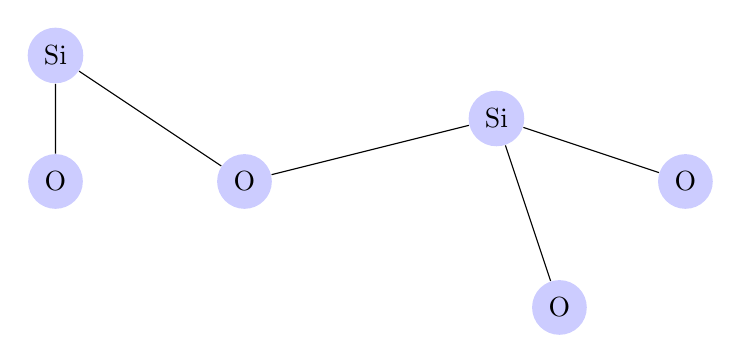
\begin{tikzpicture}
      [scale=.8,auto=left,every node/.style={circle,fill=blue!20}]
      \node (n6) at (1,10) {Si};
      \node (n4) at (4,8)  {O};
      \node (n5) at (8,9)  {Si};
      \node (n1) at (11,8) {O};
      \node (n2) at (9,6)  {O};
      \node (n7) at (1,8)  {O};
    
      \foreach \from/\to in {n6/n4,n4/n5,n5/n1,n2/n5,n6/n7}
        \draw (\from) -- (\to);
    
    \end{tikzpicture}
    \bigskip
    \\





    \item \textbf{Reduced Graph Representation}
    \\
    
    
\end{itemize}


\item \textbf{Feature Description}
\bigskip

To use ML algorithms, we want to examine features of our system such as centrality, volume, and structure.

\begin{itemize}
    \item \textbf{Centrality:} In graph theory, centrality is be used to identify the most important vertices. An example could be a specific silicon atom that is at the center of where a fracture nucleates. Identifying these vertices with the highest centrality will allow us to predict fracture nucleation.
    
    \bigskip
    
    More specifically, the vertex with the highest centrality degree would be surrounded by the most active bonds. Bonds that are not active do not necessarily contribute to the nucleation of a fracture.
    
    \begin{itemize}
        \item \textbf{Degree Centrality Measures:} We will use Degree Centrality Measures. This measure indicates how connected a vertex is by counting the direct links each vertex has to other vertices. Our network will be simplified to active bonds, therefore, the more links a vertex has to other vertices, the more connected that vertex is to active bonds. This will allow us to better understand where a fracture propagates from. 
    \end{itemize}
    
    \bigskip
    
    Additionally, we want to examine features of fracture propagation. This includes the size of a fracture and the speed of propagation. We aim to use eigenvalue centrality measure which will lend a deeper understand as to what the connections a vertex with a high degree centrality has to the entire network.
    
    \begin{itemize}
        \item \textbf{Eigenvector Centrality Measures } Eigenvector Centrality Measures indicates how much influence a specific vertex has on the entire network. For example, consider a vertex that has a high degree centrality, but does not necessarily affect the network. Therefore, it must have a low eigenvector centrality and does not contribute to a fracture that significantly damages the network. For this reason, we want to consider which vertices have a high eigenvector centrality measure in connection with degree measures. Doing so will lead us to a deeper understanding of where fractures nucleate and what the propagation of  these fractures looks like.
    \end{itemize}
\item \textbf{$Nuc_v$ and $Nuc_d$:} Within our data set are the features $nuc_v$ and $nuc_d$ which are measures of volume. By color coding our system, we are able to examine how volume gives a measure of local density. As atoms move away from one another, the local density increases. This can be visualized in our graph. Therefore, volume can help our model understand which atoms are closely associated with fracture nucleation by examining how and where volume increases.

\item\textbf{$Q_n$:} An additional feature in our data is $Q_n$ which allows us to quantify the structure. This gives rise to the connectivity of our system given that it indicates the number of oxygen atoms bonded to a silicon atom. For example, a silicon atom most commonly bonds to only four oxygen. However, it is possible to have less or more oxygen atoms bonded. Although $Q_5$ and above is generally nonphysical, conceivably it can occur due to quantum effects. 

\end{itemize}

After the model has been created, we will begin feature analysis to determine which characteristics of our system play a significant role in the accuracy of our predictions. 
\\

\item \textbf{Machine Learning Methods}
\bigskip
\\
The culminating purpose of this project is to produce a surrogate model of the molecular dynamic simulations using supervised machine learning techniques. We propose to address the our two goals listed above with address two important key outputs, predicting whether or not an atom is part of the fracture, and predicting the displacement of an atom. Note that these two outputs are discrete and continuous, respectively. Therefore this section of the methods will address our proposed ML architecture from start to finish.  

%Speak about Regression and Classification methods. 
There are two types of ML methods, classification and regression. Classification methods are machine learning algorithms whose output are a discrete set of labels whereas regression preforms a task based on independent variables and outputs a real valued number. 

%Regularization methods. LASSO , Ridge..
One concern when constructing machine learning models is the risk of \textit{overfitting} the model. A model that is overfitted will have less accuracy, and will not be able to predict due to stricter levels of flexibility when dealing with noise in the data. 




\begin{itemize}
\bigskip
\item \textbf{Method for Classifying whether or not a vertex is part of a fracture}
\bigskip
\\
%Random forest. Boosting, bagging. 
For the purpose of determining whether or not a vertex is associated with a fracture we will implement ensemble based ML methods. Ensemble classification is 


\item \textbf{Method for Predicting the Displacement of Vertices Dynamically}
\bigskip
\\

%RNN, LSTM, 

\item \textbf{Machine Learning from start to finish}
\bigskip
\\
The proposed architecture is as follows

\tikzstyle{decision} = [diamond, draw, fill=blue!20, 
    text width=4.5em, text badly centered, node distance=3cm, inner sep=0pt]
\tikzstyle{block} = [rectangle, draw, fill=blue!20, 
    text width=5em, text centered, rounded corners, minimum height=4em]
\tikzstyle{line} = [draw, -latex']
\tikzstyle{cloud} = [draw, ellipse,fill=red!20, node distance=3cm,
    minimum height=2em]
    
\begin{tikzpicture}[node distance = 2cm, auto]
    % Place nodes
    \node [block] (init) {MD Simulation Data};
    \node [block, below of=init] (features) {Extracted Features};
    \node [block, below of=features] (training) {Training Set};
    \node [block, left of=training, node distance=3cm] (test) {Test Set};
    \node [block, right of=training, node distance=3cm] (validate) {Validation Set};
    \node [decision, below of = training] (RF) {Random Forrest};
    \node [decision, below  of = test] (rnn) {RNN};
    \node [decision, below of = RF] (out) {Surrogate Model};
    %\node [cloud, below of= RF, node distance=3cm] (pof) {RF Output};
    %\node [cloud, below of= rnn, node distance=3cm] (rnnout) {RNN Output};
    
    % Draw edges
    \path [line] (init) -- (features);
    \path [line] (features) -- (validate);
    \path [line] (features) -- (training);
    \path [line] (features) -- (test);
    \path [line] (training) -- (RF);
    \path [line] (training) -- (rnn);
    \path [line] (rnn) -- (out);
    \path [line] (RF) -- (out);
    \path [line] (out) -| node [near start] {yes} (validate);
    

\end{tikzpicture}









\end{itemize}


\end{itemize}